\subsection{Segmenta��o de Imagens \label{segmentacao_de_imagens}}

Em vis�o computacional, segmenta��o � o processo de dividir uma imagem em m�ltiplas regi�es, com a inten��o de subdividir partes importantes da imagem, ou simplesmente modific�-las, ambos a fim de facilitar uma an�lise posterior. Em imagens monocrom�ticas algoritmos s�o baseados em uma das propriedades b�sicas de valores de n�veis de cinza: descontinuidade (detec��o de bordas) e similaridade (agrupamento de regi�es homog�neas). Na descontinuidade, o objetivo � particionar a imagem tendo como regra mudan�as bruscas nas escalas de cinza. A t�cnica de similaridade funciona da seguinte maneira: uma imagem f(x,y) produz como sa�da uma imagem g(x,y) , onde cada pixel da imagem f � comparado com um limiar T, se o n�vel de cinza do pixel for maior que o limiar T, este pixel � mantido em g , caso contr�rio ele � descartado (considerado como fundo). Esta t�cnica � amplamente utilizada, pois tem um baixo custo computacional.
Outra t�cnica tamb�m bastante conhecida � a limiariza��o ou binariza��o da imagem.
� dado um exemplo de histograma com limiar na Figura \ref{img_seg_histograma}:

\begin{figure}[h|top]
 \centering
 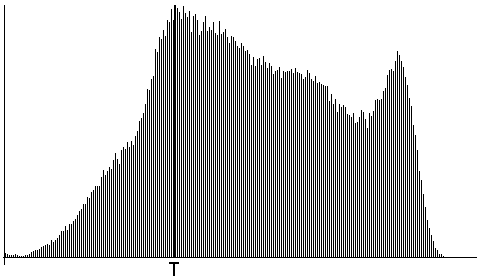
\includegraphics[width=0.5\linewidth]{imagens/seg_histograma.png}
 \caption{Exemplo de limiar com histograma.}
 \label{img_seg_histograma}
\end{figure}
 
\begin{figure}[h|top]
 \centering
 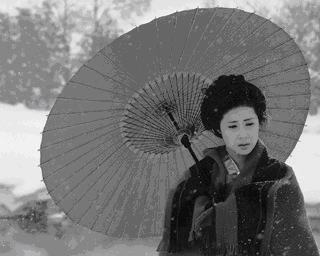
\includegraphics[width=0.5\linewidth]{imagens/seg_limiar1.png}
 \caption{Imagem Original.}
 \label{img_seg_limiar1}
\end{figure}

\begin{figure}[h|top]
 \centering
 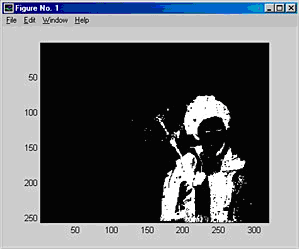
\includegraphics[width=0.5\linewidth]{imagens/seg_limiar2.png}
 \caption{Limiar = 10.}
 \label{img_seg_limiar2}
\end{figure}

\begin{figure}[h|top]
 \centering
 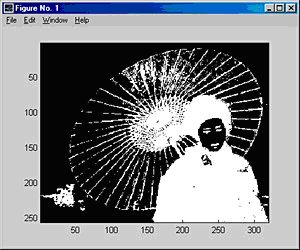
\includegraphics[width=0.5\linewidth]{imagens/seg_limiar3.png}
 \caption{Limiar = 30.}
 \label{img_seg_limiar3}
\end{figure}

\begin{figure}[h|top]
 \centering
 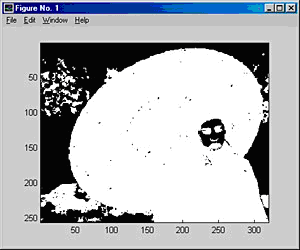
\includegraphics[width=0.5\linewidth]{imagens/seg_limiar4.png}
 \caption{Limiar = 70.}
 \label{img_seg_limiar4}
\end{figure}
 
   
Como pode ser observado nos exemplos das Figuras \ref{img_seg_limiar1} , \ref{img_seg_limiar2} , \ref{img_seg_limiar3} e \ref{img_seg_limiar4} , dependendo da limiar escolhida o resultado se altera. (explicar limiariza��o das imagens [29]).
